Sei $f \in C([a, b])$ und $Q(f) := \int_a^b f(x) dx$. Zur numerischen Approximation von $Q(f)$ seien $x_0, \ldots, x_n$ äquidistant verteilte Quadraturknoten in $[a, b]$ mit $a = x_0 < x_1 < \cdots < x_n = b$.

Es werden im weiteren Verlauf der Ausarbeitung, verschiedene summierte Quadraturformeln und deren Zusammenhänge untersucht.

\subsection{Die summierte Trapez-Regel}

Die Menge aller zulässigen Abstände zwischen beliebig äquidistanten Quadraturknoten, bezeichnen wir mit $H := \Bbraces{\frac{b-a}{n}: n \in \N}$. Somit, können wir, für fixes $h \in H$, diese $x_0, \ldots, x_n$ durch $x_i := a + hi$, $i = 1, \ldots, n$, charakterisieren. Man verifiziert unmittelbar, dass

\begin{align*}
    x_0 = a, \,
    x_n = b, \quad
    \Forall i = 1, \ldots, n:
    x_i - x_{i-1} = h.
\end{align*}

Wir beginnen damit, die ersten paar abgeschlossenen Newton-Cotes-Formeln auszurechnen. Diese ergeben sich bekanntlich aus dem lagrange'schen Interpolationspolynom $p_f \in \Pi_n$ von $f$.

\begin{align*}
    Q^{(n)}(f)
    = \int_a^b p_f(x) dx
    = \int_a^b \sum_{i=0}^n f(x_i) L_i(x) dx
    = \sum_{i=0}^n f(x_i) \int_a^b L_i(x) dx
\end{align*}

\begin{align*}
    L_i(x) :=
    \prod_{\substack{j=0 \\ j \neq i}}^n
    \frac{x - x_j}{x_i - x_j}, \quad
    i = 0, \ldots, n
\end{align*}

Nachdem die Lagrange Basis Polynome $L_j$, $j = 0, \ldots, n$, umständlich zu integrieren sind, wird hier nicht per Hand, sondern mit dem Python-Paket SymPy gearbeitet.

\inputminted{python}{Aufgabe_2/python_code/newton_cotes_formeln.py}

Damit errechnet man jeweils die Trapez-, Simpson- und Mile-Regel.

\begin{align*}
    Q^{(1)}(f) \label{trapezium}
    & = \frac{b-a}{2}
        \pbraces
        {
            f(a) +
            f(b)
        } \\
    Q^{(2)}(f) \label{simpson}
    & = \frac{b-a}{6}
        \pbraces
        {
            f(a) +
            4 f \pbraces{\frac{a+b}{2}} +
            f(b)
        } \\
    Q^{(4)}(f) \label{mile}
    & = \frac{b-a}{90}
        \pbraces
        {
            7  f(a) + 
            32 f \pbraces{\frac{3a+b}{4}} +
            12 f \pbraces{\frac{a+b}{2}} +
            32 f \pbraces{\frac{a+3b}{4}} +
            7  f(b)
        }
\end{align*}

Jetzt können auch die jeweils summierten Quadraturformeln bestimmt werden. Wir setzen uns vorerst nur mit der Summierten Trapez-Regel $Q_\cdot^{(1)}(f): H \to \K$ auseinander.

\begin{align*}
    Q_h^{(1)}(f)
    & = \sum_{i=1}^n Q^{(1)}(f|_{[x_{i-1}, x_i]}) \\
    & = \sum_{i=1}^n
        \frac{x_i - x_{i-1}}{2}
        \pbraces
        {
            f(x_{i-1}) +
            f(x_i)
        } \\
    & = \frac{h}{2}
        \pbraces
        {
            \sum_{i=1}^n f(x_{i-1}) +
            \sum_{i=1}^n f(x_i)
        } \\
    & = \frac{h}{2}
        \pbraces
        {
            f(x_0) +
            \sum_{i=2}^n f(x_{i-1}) +
            \sum_{i=1}^{n-1} f(x_i) +
            f(x_n)
        } \\
    & = \frac{h}{2}
        \pbraces
        {
            f(a) +
            2 \sum_{i=1}^{n-1} f(x_i) +
            f(b)
        } \\
\end{align*}

Wir wollen nun den Quadraturfehler der summierten Trapez-Regel genauer zu untersuchen.

\begin{align*}
    \epsilon_h^{(1)} := \vbraces{Q - Q_h^{(1)}}
\end{align*}

Dazu definieren wir uns eine Folge von Testfunktionen $g_k(x) := \sqrt{x}^k$, $k \in \N$. Deren Stammfunktionen sind offensichtlich $(\int g_k)(x) = \frac{2}{k+2} \sqrt{x}^{k+2}$. Die summierte Trapezregel $Q_\cdot^{(1)}$ zu implementieren, ist ebenso schnell geschafft. Damit können wir auch schon den Quadraturfehler $\epsilon^{(1)}_\cdot(g_k)$, explizit berechnen lassen. \\

\inputminted{python}{Aufgabe_2/python_code/summierte_trapez_regel.py}

Dieser wurde in Abbildung \ref{fig:konvergenz_plot_1} auf $\Bbraces{\frac{b-a}{n}: n = 1, \ldots, 16} \subset H$, für $k = 1, 3, 4$, auf beiden Achsen logarithmisch, geplottet. Dabei werden $g_0$ und $g_2$ sind nicht abgebildet, weil sie, als Lineare Funktionen, offensichtlich sofort, durch $Q^{(1)}$ bzw. $Q_h^{(1)}$, exakt berechnet werden. Das macht sie für die folgende Analyse uninteressant. Auch $g_k$, $k \geq 5$, werden ausgelassen, da sie, bezüglich Konvergenzverhalten, keine markanten Unterschiede zu $g_4$ aufweisen. $\text{id}^{-2}$ ist dabei eine Referenzfunktion für das Konvergenzverhalten.

\begin{figure}[H]
\centering
\subfloat[$a = 0$, $b = 1$]{
  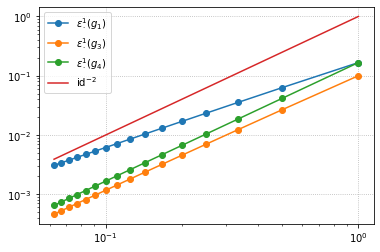
\includegraphics[width=65mm]{Aufgabe_2/latex_code/images/konvergenz_plot_1_1.png}
}
\subfloat[$a = \frac{1}{2}$, $b = 1$]{
  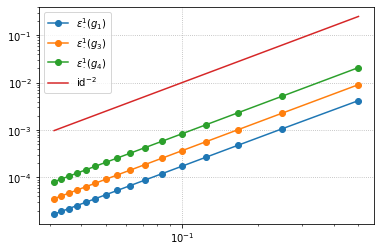
\includegraphics[width=65mm]{Aufgabe_2/latex_code/images/konvergenz_plot_1_2.png}
}
\hspace{0mm}
\caption{Konvergenzverhalten von $\epsilon_\cdot^{(1)}(g_k)$, $k = 1, 3, 4$ auf $[a, b]$}
\label{fig:konvergenz_plot_1}
\end{figure}

Es scheinen also $g_3$ und $g_4$, quadratisch zu konvergieren, d.h. $\epsilon_h^{(1)}(g_k) = \Landau{h^2}$, $h \to \infty$, $k = 3, 4$. Abbildung \ref{fig:konvergenz_plot_1} ist auch zu entnehmen, dass $\epsilon_h^{(1)}(g_1)$ langsamer konvergiert. Es stellt sich heraus, dass dieses Phänomen auch bereits bei $a \approx 0$ auftritt. \\

Um das zu erklären, betrachten wir $g_1$ im Intervall $[0, 1]$. Der Quadraturfehler $\epsilon_h^{(1)}(g_1)$ dieser Funktion wird dazu auf $n$ Intervalle der Länge $h$ aufgeteilt. Man beachte, dass darauf die normale Trapez-Regel $Q^{(1)}$ gilt. \\

\begin{align} \label{partition}
    [0, 1] = \bigcup_{i=0}^{n-1} [hi, h(i+1)]
\end{align}

Der erste Fehler $\epsilon_h^{(1)}(g_1|_{[0, h]})$ muss direkt über die Stammfunktion von $g_1$ bestimmt werden.

\begin{multline*}
    \epsilon_h^{(1)}(g_k|_{[0, h]})
    =   \vbraces
        {
            Q(g_1|_{[0, h]}) -
            Q^{(1)}(g_1|_{[0, h]})
        } \\
    =   \frac{2}{1+2}
        \sqrt{x}^{1+2} \Big |_0^h -
        \frac{h-0}{2} \pbraces{\sqrt{0}^1 + \sqrt{h}^1}
    =   \frac{2}{3} \sqrt{h}^3 -
        \frac{1}{2} \sqrt{h}^3
    =   \frac{1}{6} \sqrt{h}^3
\end{multline*}

Für die anderen Fehler $\epsilon_h^{(1)}(g_1|_{[hi, h(i+1)]})$, braucht man die zweiten Ableitungen $g_1''$. Dabei ist $i = 1, \ldots, n-1$.

\begin{align*}
    \frac{d^2}{dx^2} g_1(x)
    = \frac{d^2}{d^2x} x^{\frac{1}{2}}
    = \frac{1}{2} \frac{d}{dx} x^{-\frac{1}{2}}
    = - \frac{1}{4} x^{-\frac{3}{2}}
    = - \frac{1}{4 \sqrt{x}^3}
\end{align*}

Nachdem $|g_1''|$ monoton fällt, muss $\norm[\infty]{g_1''|_{[hi, h(i+1)]}} = \vbraces{g_1''(hi)} = \frac{1}{4 \sqrt{hi}^3}$. Somit erhalten wir eine Fehlerabschätzung mit $\Exists \xi \in (hi, h(i+1)):$

\begin{multline*}
    \epsilon_h^{(1)}(g_k|_{[hi, h(i+1)]})
    =   \vbraces
        {
            Q(g_1|_{[hi, h(i+1)]}) -
            Q^{(1)}(g_1|_{[hi, h(i+1)]})
        } \\
    =   \vbraces
        {
            - \frac{(h(i+1) - hi)^3}{12}
            g_1''|_{[hi, h(i+1)]}(\xi)
        }
      \leq
        \frac{h^3}{12}
        \norm[\infty]{g_1''|_{[hi, h(i+1)]}}
    =   \frac{h^3}{12}
        \frac{1}{4 \sqrt{hi}^3}
    =   \frac{\sqrt{h}^3}{48 \sqrt{i}^3}
\end{multline*}

Wir setzen die einzelnen zum Fehler, laut \eqref{partition}, auf das gesamte Intervall $[0, 1]$ zusammen.

\begin{align*}
    \epsilon_h^{(1)}(g_1)
    & = \vbraces
        {
            Q(g_1) - Q_h^{(1)}(g_1)
        }
    =   \vbraces
        {
            \sum_{i=0}^{n-1} Q(g_1|_{[hi, h(i+1)]}) -
            \sum_{i=0}^{n-1} Q^{(1)}(g_1|_{[hi, h(i+1)]})
        } \\
    & \leq
        \sum_{i=0}^{n-1} \vbraces
        {
            Q(g_1|_{[hi, h(i+1)]}) -
            Q^{(1)}(g_1|_{[hi, h(i+1)]})
        }
    =   \epsilon_h^{(1)}(g_1|_{[0, h]}) +
        \sum_{i=1}^{n-1} \epsilon_h^{(1)}(g_1|_{[hi, h(i+1)]}) \\
    & \leq
        \frac{1}{6} \sqrt{h}^3 +
        \sum_{i=1}^{n-1} \frac{\sqrt{h}^3}{48 \sqrt{i}^3}
    =   \underbrace
        {
            \frac{1}{6}
            \pbraces
            {
                1 + \frac{1}{8} \sum_{i=1}^{n-1} \frac{1}{i^\frac{3}{2}}
            }
        }_{ =: \, C}
        \sqrt{h}^3
\end{align*}

Weil $C < \infty$, und die Abschätzung für kleines $h$ scharf ist bekommt man also tatsächlich keine quadratische Konvergenz.

\begin{align*}
    \epsilon_h^{(1)}(g_1)
    \approx
    \Landau{\sqrt{h}^3}, \quad
    h \to 0
\end{align*}

\subsection{Die summierte Simpson- und Mile-Regel}

Es wird, ohne Beweis, vorausgesetzt, dass die summierte Trapez-Regel $Q_\cdot^{(1)}(f)$, eine asymptotische Entwicklung besitzt.

\begin{align} \label{asymptotisch}
    Q_h^{(1)}(f) =
    Q(f) +
    \sum_{i=1}^r a_i h^{2i} +
    a_{r+1}(h)
    \quad \text{ mit }
    a_{r+1}(h) = \Landau{h^{2r+2}}
    \text{ für }
    h \to 0.
\end{align}

Wir wollen nämlich eine lineare Richardson-Extrapolation, mit der Romberg-Folge $(h_k)_{k \in \N_0}$, auf die summierte Trapez-Regel $Q_\cdot^{(1)}(f)$ anwenden.

\begin{align*}
    h_0 \in H, \quad
    h_k := \frac{h_0}{2^k}, \quad
    n_k := \frac{b-a}{h_k}, \quad
    k \in \N_0
\end{align*}

Diese Art von Folge, wo das vorherige Glied ganzzahlig geteilt wird, wird sich als überaus nützlich erweisen. Das lässt nämlich eine Wiederverwertung von Funktionsauswertungen an den vorherigen Stützstellen zu. \\

Man verifiziert unmittelbar die nützlichen Eigenschaften $\Forall k, \ell \in \N_0:$

\begin{align*}
    \frac{h_{k + \ell}}{h_k} = \frac{1}{2^\ell}, \quad
    n_k = 2^k n_0.
\end{align*}

Für $i = 0, \ldots, n_0$ und $j = 0, \ldots, n_1$, brauchen $Q_{h_0}^{(1)}$ und $Q_{h_1}^{(1)}$ noch die Quadraturknoten $x_i := a + h_0 i$ und $y_i := a + h_1 j$. Durch Einsetzen und elementares Nachrechnen, ergeben sich die Eigenschaften $\Forall i = 1, \ldots, n_0:$

\begin{align*}
    y_{2i - 1} = \frac{x_{i-1} + x_i}{2}, \quad
    y_{2i} = x_i.
\end{align*}

Es wird, für die Extrapolation, ein Ausschnitt des Neville-Aitken Schemas benutzt.

\begin{align*}
\begin{array}{ccc}
    Q_{h_0}^{(1)}(f) = a_{0,0}
    && \\
    & \searrow & \\
    Q_{h_1}^{(1)}(f) = a_{1,0}
    & \rightarrow &
    a_{0,1}
    = a_{0,0} +
      \frac
      {a_{0,0} - a_{1,0}}
      {\pbraces{\frac{h_1}{h_0}}^2 - 1}
\end{array}
\end{align*}

Man erkennt, dass eine lineare Extrapolation der summierten Trapez-Regel $Q_\cdot^{(1)}(f)$, genau in der summierten Simpson-Regel $Q_\cdot^{(2)}(f)$ resultiert.

\begin{align*}
    a_{0,1}
    & = Q_{h_0}^{(1)}(f) +
        \frac
        {Q_{h_0}^{(1)}(f) - Q_{h_1}^{(1)}(f)}
        {\pbraces{\frac{1}{2}}^2 - 1} \\
    & = \frac{1}{3}
        \pbraces
        {
            - Q_{h_0}^{(1)}(f)
            + 4 Q_{h_1}^{(1)}(f)
        } \\
    & = \frac{1}{3}
        \pbraces
        {
            - \frac{h_0}{2}
            \pbraces
            {
                f(a) +
                2 \sum_{i=1}^{n_0 - 1} f(x_i) +
                f(b)
            }
            + 4 \frac{h_1}{2}
            \pbraces
            {
                f(a) +
                2 \sum_{i=1}^{n_1 - 1} f(y_i) +
                f(b)
            }
        } \\
    & = \frac{1}{3}
        \pbraces
        {
            - \frac{h_0}{2}
            \pbraces
            {
                f(a) +
                2 \sum_{i=1}^{n_0 - 1} f(x_i) +
                f(b)
            }
            + \frac{2 h_0}{2}
            \pbraces
            {
                f(a) +
                2 \sum_{i=1}^{2 n_0 - 1} f(y_i) +
                f(b)
            }
        } \\
    & = \frac{h_0}{3}
        \pbraces
        {
            - \frac{1}{2}
            \pbraces
            {
                f(a) +
                2 \sum_{i=1}^{n_0 - 1} f(x_i) +
                f(b)
            }
            + \pbraces
            {
                f(a) +
                2 \pbraces
                {
                    \sum_{i=1}^{n_0} f(y_{2i-1}) +
                    \sum_{i=1}^{n_0-1} f(y_{2i})
                } +
                f(b)
            }
        } \\
    & = \frac{h_0}{3}
        \pbraces
        {
            - \frac{1}{2}
            \pbraces
            {
                f(a) +
                2 \sum_{i=1}^{n_0 - 1} f(x_i) +
                f(b)
            }
            + \pbraces
            {
                f(a) +
                2 \pbraces
                {
                    \sum_{i=1}^{n_0}
                    f \pbraces{\frac{x_{i-1} - x_i}{2}} +
                    \sum_{i=1}^{n_0-1} f(x_i)
                } +
                f(b)
            }
        } \\
    & = \frac{h_0}{6}
        \pbraces
        {
            f(a) +
            4 \sum_{i=1}^{n_0}
            f \pbraces{\frac{x_{i-1} - x_i}{2}} +
            2 \sum_{i=1}^{n_0 - 1} f(x_i) +
            f(b)
        } \\
    & = Q_{h_0}^{(2)}(f)
\end{align*}

Man könnte erwarten, dass eine quadratische Extrapolation zur summierten $3/8$-Regel $Q_\cdot^{(3)}(f)$ führt. Aufgrund der Wahl der Folge $(h_k)_{k \in \N_0}$, ist die summierte Mile-Regel, $Q_\cdot^{(4)}(f)$, aber ein plausiblerer Kandidat. Um diese Vermutungen zu überprüfen, befleißigen wir uns abermals am Neville-Aitken Schema.

\begin{align*}
\begin{array}{ccccc}
    Q_{h_0}^{(1)}(f) = a_{0,0}
    &&&& \\
    & \searrow &&& \\
    Q_{h_1}^{(1)}(f) = a_{1,0}
    & \rightarrow &
    a_{0,1}
    = a_{0,0} + \frac{a_{0,0} - a_{1,0}}{\pbraces{\frac{h_1}{h_0}}^2 - 1}
    && \\
    & \searrow && \searrow & \\
    Q_{h_2}^{(1)}(f) = a_{2,0}
    & \rightarrow &
    a_{1,1}
    = a_{1,0} + \frac{a_{1,0} - a_{2,0}}{\pbraces{\frac{h_2}{h_1}}^2 - 1}
    & \rightarrow &
    a_{0,2}
    = a_{0,1} + \frac{a_{0,1} - a_{1,1}}{\pbraces{\frac{h_2}{h_0}}^2 - 1} \\
\end{array}
\end{align*}

Es ist ja, durch die lineare Extrapolation, bereits bekannt, dass $a_{0,1} = Q_{h_0}^{(2)}(f)$. Man kann aber sogar, durch die selbe Rechnung, nur mit geshifteten $h_0 \mapsto h_1 \mapsto h_2$, auch auf $a_{1,1} = Q_{h_1}^{(2)}(f)$ kommen. \\

Durch nochmaliges Einsetzen und elementares Nachrechnen, ergeben sich wiederum $\Forall i = 1, \ldots, n_0:$

\begin{align*}
    \frac{y_{2i - 2} + y_{2i - 1}}{2}
    = \frac{3 x_{i-1} + x_i}{4}, \quad
    \frac{y_{2i - 1} + y_{2i}}{2}
    = \frac{x_{i-1} + 3 x_i}{4}.
\end{align*}

Die Annahme, dass eine quadratische Extrapolation der summierten Trapez-Regel $Q_\cdot^{(1)}(f)$ die summierte Mile-Regel $Q_\cdot^{(4)}(f)$ liefert, wird hiermit bestätigt.

\begin{align*}
    & a_{0,2} \\
    & = Q_{h_0}^{(2)}(f) +
        \frac
        {Q_{h_0}^{(2)}(f) - Q_{h_1}^{(2)}(f)}
        {\pbraces{\frac{1}{2^2}}^2 - 1} \\
    & = \frac{1}{15}
        \pbraces
        {
            - Q_{h_0}^{(2)}(f)
            + 16 Q_{h_1}^{(2)}(f)
        } \\
    & = \frac{1}{15}
        \Bigg (
            - \frac{h_0}{6}
            \pbraces
            {
                f(a) +
                2 \sum_{i=1}^{n_0 - 1} f(x_i) +
                4 \sum_{i=1}^{n_0} f \pbraces{\frac{x_{i-1} + x_i}{2}} +
                f(b)
            } \\
    & +
            16 \frac{h_1}{6}
            \pbraces
            {
                f(a) +
                2 \sum_{i=1}^{n_1 - 1} f(y_i) +
                4 \sum_{i=1}^{n_1} f \pbraces{\frac{y_{i-1} + y_i}{2}} +
                f(b)
            }
        \Bigg ) \\
    & = \frac{1}{15}
        \Bigg (
            - \frac{h_0}{6}
            \pbraces
            {
                f(a) +
                2 \sum_{i=1}^{n_0 - 1} f(x_i) +
                4 \sum_{i=1}^{n_0} f \pbraces{\frac{x_{i-1} + x_i}{2}} +
                f(b)
            } \\
    & +
            \frac{8 h_0}{6}
            \pbraces
            {
                f(a) +
                2 \sum_{i=1}^{2 n_0 - 1} f(y_i) +
                4 \sum_{i=1}^{2 n_0} f \pbraces{\frac{y_{i-1} + y_i}{2}} +
                f(b)
            }
        \Bigg ) \\
    & = \frac{h_0}{90}
        \Bigg (
            - \pbraces
            {
                f(a) +
                2 \sum_{i=1}^{n_0 - 1} f(x_i) +
                4 \sum_{i=1}^{n_0} f \pbraces{\frac{x_{i-1} + x_i}{2}} +
                f(b)
            } \\
    & +
            8 \pbraces
            {
                f(a) +
                2 \pbraces
                {
                    \sum_{i=1}^{n_0} f(y_{2i-1}) +
                    \sum_{i=1}^{n_0 - 1} f(y_{2i})
                } +
                4 \pbraces
                {
                    \sum_{i=1}^{n_0} f \pbraces{\frac{y_{2i-2} + y_{2i-1}}{2}} +
                    \sum_{i=1}^{n_0} f \pbraces{\frac{y_{2i-1} + y_{2i}}{2}}
                } +
                f(b)
            }
        \Bigg ) \\
    & = \frac{h_0}{90}
        \Bigg (
            - \pbraces
            {
                f(a) +
                2 \sum_{i=1}^{n_0 - 1} f(x_i) +
                4 \sum_{i=1}^{n_0} f \pbraces{\frac{x_{i-1} + x_i}{2}} +
                f(b)
            } \\
    & +
            8 \pbraces
            {
                f(a) +
                2 \pbraces
                {
                    \sum_{i=1}^{n_0} f \pbraces{\frac{x_{i-1} - x_i}{2}} +
                    \sum_{i=1}^{n_0 - 1} f(x_i)
                } +
                4 \pbraces
                {
                    \sum_{i=1}^{n_0} f \pbraces{\frac{3 x_{i-1} + x_i}{4}} +
                    \sum_{i=1}^{n_0} f \pbraces{\frac{x_{i-1} + 3 x_i}{4}}
                } +
                f(b)
            }
        \Bigg ) \\
    & = \frac{h_0}{90}
        \Bigg (
            - \pbraces
            {
                f(a) +
                2 \sum_{i=1}^{n_0 - 1} f(x_i) +
                4 \sum_{i=1}^{n_0} f \pbraces{\frac{x_{i-1} + x_i}{2}} +
                f(b)
            } \\
    & +
            8 \pbraces
            {
                f(a) +
                2 \pbraces
                {
                    \sum_{i=1}^{n_0} f \pbraces{\frac{x_{i-1} - x_i}{2}} +
                    \sum_{i=1}^{n_0 - 1} f(x_i)
                } +
                4 \pbraces
                {
                    \sum_{i=1}^{n_0} f \pbraces{\frac{3 x_{i-1} + x_i}{4}} +
                    \sum_{i=1}^{n_0} f \pbraces{\frac{x_{i-1} + 3 x_i}{4}}
                } +
                f(b)
            }
        \Bigg ) \\
    & = \frac{h_0}{90}
        \pbraces
        {
            7 f(a) +
            32 \sum_{i=1}^{n_0} f \pbraces{\frac{3 x_{i-1} + x_i}{4}} +
            12 \sum_{i=1}^{n_0} f \pbraces{\frac{x_{i-1} + x_i}{2}} +
            14 \sum_{i=1}^{n_0 - 1} f(x_i) +
            32 \sum_{i=1}^{n_0} f \pbraces{\frac{x_{i-1} + 3 x_i}{4}} +
            7 f(b)
        } \\
    & = Q_{h_0}^{(4)}(f)
\end{align*}

Uns interessiert natürlich wieder das Konvergenzverhalten der eben extrapolierten Regeln. Dazu implementieren wir diesmal die summierte Simpson-Regel $Q_\cdot^{(2)}$ und Mile-Regel $Q_\cdot^{(4)}$.

\inputminted{python}{Aufgabe_2/python_code/summierte_simpson_regel.py}
\inputminted{python}{Aufgabe_2/python_code/summierte_mile_regel.py}

Um die Quadraturfehler der summierten Simpson-Regel $\epsilon_h^{(2)}$ und Mile-Regel $\epsilon_h^{(4)}$ zu untersuchen, wurden wieder Konvergenzplots, analog zu Abbildung \ref{fig:konvergenz_plot_1} erstellt.

\begin{figure}[H]
\centering
\subfloat[$a = 0$, $b = 1$]{
  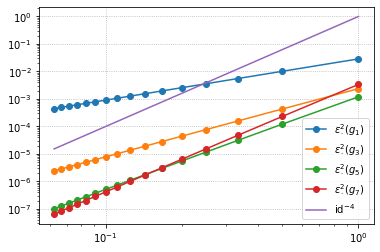
\includegraphics[width=65mm]{Aufgabe_2/latex_code/images/konvergenz_plot_2_1.png}
}
\subfloat[$a = \frac{1}{2}$, $b = 1$]{
  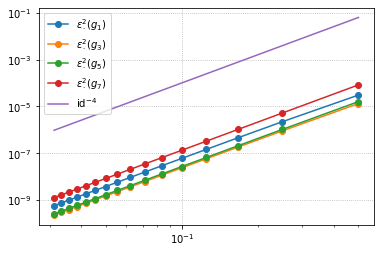
\includegraphics[width=65mm]{Aufgabe_2/latex_code/images/konvergenz_plot_2_2.png}
}
\hspace{0mm}
\caption{Konvergenzverhalten von $\epsilon_\cdot^{(2)}(g_k)$, $k = 1, 3, 5, 7$ auf $[a, b]$}
\label{fig:konvergenz_plot_2}
\end{figure}
\begin{figure}[H]
\centering
\subfloat[$a = 0$, $b = 1$]{
  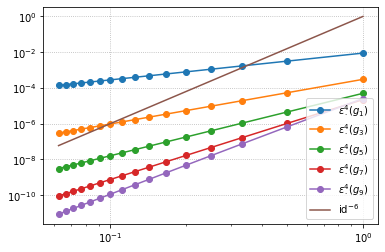
\includegraphics[width=65mm]{Aufgabe_2/latex_code/images/konvergenz_plot_3_1.png}
}
\subfloat[$a = \frac{1}{2}$, $b = 1$]{
  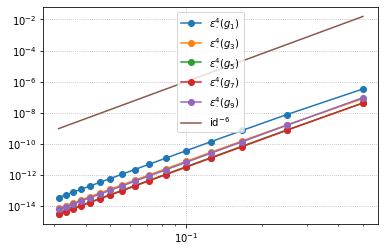
\includegraphics[width=65mm]{Aufgabe_2/latex_code/images/konvergenz_plot_3_2.png}
}
\hspace{0mm}
\caption{Konvergenzverhalten von $\epsilon_\cdot^{(4)}(g_k)$, $k = 1, 3, 5, 7, 9$ auf $[a, b]$}
\label{fig:konvergenz_plot_3}
\end{figure}

Es stellt sich wieder die berechtigte Frage, wie es zu diesen Ergebnissen kommen kann, und ob es einen Zusammenhang zum Quadraturfehler der summierten Trapezregel $\epsilon_h^{(1)}$ geben könnte. Die Antwort wird im nächsten Abschnitt gleich ganz allgemein beantwortet. \\

Um den unpassenden Quadraturfehler der summierten Simpson-Regel $\epsilon_\cdot^{(2)}(g_k)$, $k = 1, 3, 5$, zu erklären, kann man analog zum vorherigen Abschnitt vorgehen. Dazu eignet sich wieder die Partition \eqref{partition} und, etwas andere, Restglieddarstellung der Simpson-Regel auf den einzelnen Teilintervallen. \\

\begin{align*}
    \Forall i = 1, \ldots, n-1:
    \Exists \xi \in (hi, h(i+1)):
    Q(f) - Q^{(2)}(f)
      = - \frac{(h(i+1) - hi)^5}{2880} f^{(4)}(\xi)
      = - \frac{h^5}{2880} f^{(4)}(\xi)
\end{align*}

\subsection{Höhere Quadraturformeln}

Zuletzt, werden wir noch eine allgemeine Richardson-Extrapolation der summierten Trapez-Regel $Q_\cdot^{(1)}$ formulieren und implementerien.

\begin{align}
\begin{array}{cccccc}
    Q_{h_0}^{(1)}(f) = a_{0,0}
    &&&&& \\
    & \searrow &&&& \\
    Q_{h_1}^{(1)}(f) = a_{1,0}
    & \rightarrow &
    a_{0,1}
    &&& \\
    & \searrow && \searrow && \\
    Q_{h_2}^{(1)}(f) = a_{2,0}
    & \rightarrow &
    a_{1,1}
    & \rightarrow &
    a_{0,2}
    & \\
    \vdots & \vdots & \vdots & \vdots & \vdots & \ddots
\end{array}
\label{neville_aitken}
\end{align}

\begin{align}
    a_{j, 0}
    & = Q_{h_j}^{(1)}(f),
    & j \in \N_0
    \label{rekursions_basis} \\
    a_{j, i}
    & = a_{j, i-1} +
    \frac
    {
        a_{i, i-1} -
        a_{j+1, i-1}
    }{
        \pbraces
        {
            \frac
            {
                h_{j+i}
            }{
                h_j
            }
        }^2 -
        1
    },
    & i \in \N, \quad j \in \N_0
    \label{rekursions_schritt}
\end{align}


Die wohl einfachste bzw. naheliegendste Implementierung der Richardson Extrapolation ist wahrscheinlich rekursiv. Um Rekursionszweige zu sparen, kann man Hilfsvariablen einführen, anstatt die Rekursionsformel in einem Aufwaschen auswerten zu lassen.

\inputminted{python}{Aufgabe_2/python_code/ineffiziente_extrapolation.py}

Trotz Hilfsvariablen, ist die obere eine miserable Implementierung. Sie ist deswegen so schlecht, weil die Einträge der rechten Spalte, also die Rekursionsbasis \eqref{rekursions_basis}, vom Neville-Aitken Schema \eqref{neville_aitken}, jedes Mal separat berechnet werden. \\

Weitaus sparsamer, was Funktionsauswertungen angeht, kann man mit Loops davonkommen. Dazu wird bei $a_{0,0} = Q_{h_0}^{(1)}(f)$, oben rechts in \eqref{neville_aitken}, gestartet und, mit dem gespeicherten Ergebnis, der darunterliegenden Eintrag $a_{1,0} = Q_{h_1}^{(1)}(f)$ berechnet.

\begin{align*}
    Q_{h_1}^{(1)}(f)
    & = \frac{h_1}{2}
        \pbraces
        {
            f(a) +
            2 \sum_{i=1}^{n_1 - 1} f(y_i) +
            f(b)
        } \\
    & = \frac{h_0}{4}
        \pbraces
        {
            f(a) +
            2 \sum_{i=1}^{2 n_0 - 1} f(y_i) +
            f(b)
        } \\
    & = \frac{h_0}{4}
        \pbraces
        {
            f(a) +
            2 \pbraces
            {
                \sum_{i=1}^{n_0 - 1} f(y_{2i}) +
                \sum_{i=1}^{n_0} f(y_{2i-1})
            }
            f(b)
        } \\
    & = \frac{h_0}{4}
        \pbraces
        {
            f(a) +
            2 \pbraces
            {
                \sum_{i=1}^{n_0 - 1} f(x_i) +
                \sum_{i=1}^{n_0} f \pbraces{\frac{x_{i-1} - x_i}{2}}
            } +
            f(b)
        } \\
    & = \frac{1}{2}
        \pbraces
        {
            \frac{h_0}{2}
            \pbraces
            {
            f(a) +
            2 \sum_{i=1}^{n_0 - 1} f(x_i) +
            f(b)
            } +
            h_0 \sum_{i=1}^{n_0} f \pbraces{\frac{x_{i-1} - x_i}{2}}
        } \\
    & = \frac{1}{2}
        \pbraces
        {
            Q_{h_0}^{(1)}(f) +
            h_0 \sum_{i=1}^{n_0} f \pbraces{\frac{x_{i-1} - x_i}{2}}
        }
    \label{effiziente_extrapolation}
\end{align*}

Das wird so lange fortgesetzt, bis hinreichend viele Einträge berechnet wurden. Den Rest darf dann aber der Rekursionsschritt \eqref{rekursions_schritt} erledigen.

\inputminted{python}{Aufgabe_2/python_code/effiziente_extrapolation.py}

Ein drittes und letztes Mal, wollen wir über das Konvergenzverhalten bescheid wissen. Dazu verifizieren wir die Voraussetzungen des Satzes zum Extrapolationsfehler. \\

Die asymptotische Entwicklung \eqref{asymptotisch} der summierten Trapez-Regel $Q_\cdot^{(1)}(f): H \to \K$ lässt sich in folgende Form umschreiben.

\begin{align*}
    Q_h^{(1)}(f) =
    Q(f) +
    \sum_{i=1}^r a_i h^{iq} +
    a_{r+1}(h) h^{(r+1) q}, \quad
    h > 0, \quad
    a_{r+1}(h)
    = a_{r+1} + \landau{1}, \quad
    h \to 0
\end{align*}

Für unsere Folge $(h_k)_{k \in \N_0}$ aus $\R_{>0}^{\N_0}$ gilt mit $\rho \in [\frac{1}{2}, 1)$ auch $0 < \frac{h_{k+1}}{h_k} \leq \rho < 1$. Sei dann noch $p_r^{(k)} \in \Pi_r$ das interpolierende Polynom mit

\begin{align*}
    p_r^{(k)} \pbraces{h_{k+j}^q}
    = Q_{h_{k+j}}^{(1)}(f), \quad
    j = 0, \ldots, r.
\end{align*}

Somit erhält man für den Extrapolationsfehler, mit $Q = Q_0^{(1)}$ und $a_{k, r} = p_r^{(k)}(0)$, folgendes Ergebnis. Dabei entspricht $r$ wieder dem Extrapolationsgrad und $k$ ist der Index unser obigen Folge $(h_k)_{k \in \N_0}$.

\begin{align}
    Q(f) - a_{k, r}
    = \Landau{h_k^{2r+2}}, \quad
    k \to \infty
    \label{extrapolationsfehler}
\end{align}

\eqref{extrapolationsfehler} vereinigt die, in Abbildung \ref{fig:konvergenz_plot_1} bis \ref{fig:konvergenz_plot_3} aufgetretenen, Konvergenzverhalten der summierten Trapez- bis Mile-Regel. Das wird in der folgenden Abbildung \ref{fig:konvergenz_plot_4} nochmals veranschaulicht. Die Testfunktion $f: x \mapsto \sin{\pi x}$ hat dabei offensichtlich die Stammfunktion $(\int f)(x) = - \frac{1}{\pi} \cos{\pi x}$ und die Steigungen entsprechen genau den Potenzen von \eqref{extrapolationsfehler}.

\begin{figure}[H]
\centering
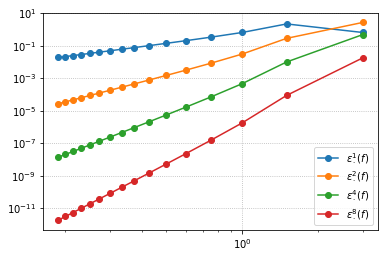
\includegraphics[width=65mm]{Aufgabe_2/latex_code/images/konvergenz_plot_4.png}
\caption{Konvergenzverhalten von $\epsilon_\cdot^{(m)}(f)$, $m = 2^r$, $r = 0, \ldots, 3$, auf $[0, 1]$}
\label{fig:konvergenz_plot_4}
\end{figure}

Zuletzt vergleichen wir noch die diversen Quadraturen $Q_h^{(m)}$ bezüglich der Anzahl der benötigten Funktionsauswertungen $\# Q_h^{(m)}$. \\

Zunächst einmal, kann man für die summierte Trapez-, Simpson, und Mile-Regel unmittelbar ablesen, dass $\# Q_h^{(m)} = nm + 1$, $m = 1, 2, 4$. \\

Bei der ineffizienten Extrapolation, werden die Ergebnisse von $Q_{h_{j-1}}^{(1)}$ nicht für die Berechnung von $Q_{h_j}^{(1)}$ wieder-verwertet. Bei einem Extrapolationsgrad von $r$, sind also dementsprechend viele Funktionsauswertungen zu erwarten.

\begin{align*}
    \# Q_{h_0}^{(2^r)}
    = \sum_{j=0}^r \# Q_{h_j}^{(1)}
    = \sum_{j=0}^r n_j + 1
    = n_0 \sum_{j=0}^r 2^j + \sum_{j=0}^r 1
    = n_0 (2^{r+1} - 1) + r + 1
\end{align*}

Die effizientere Implementierung der Extrapolation, liegt hingegen deutlich im Vorteil. Die summierte Trapez-, Simpson, und Mile-Regel passen hier offensichtlich, mit $m(r) = 2^r$, ebenfalls ins Schema.

\begin{align*}
    \# Q_{h_0}^{(2^r)}
    = \# Q_{h_0}^{(1)} + \sum_{j=1}^r n_{j-1}
    = n_0 + 1 + \sum_{j=0}^{r-1} n_j
    = n_0 + 1 + n_0 \sum_{j=0}^{r-1} 2^j
    = n_0 + 1 + n_0 (2^r - 1)
    = n_0 2^r + 1
\end{align*}

Wenn wir uns nun von der ursprünglichen Grundmenge $H$ der summierten Quadraturformeln $Q_\cdot^{(m)}(f)$ auf die Romberg-Folge $\Bbraces{h_k: k \in \N_0}$ einschränken, so erhalten wir, laut \eqref{extrapolationsfehler}, sogar exponentielle Konvergenz mit der Basis $2$. Das hat natürlich seinen Preis. Zwar können die Ergebnisse der Funktionsauswertungen durch diese Folge, wie wir gesehen haben, wieder verwertet werden. Das ändert aber nichts an der Tatsache, dass die Gesamtanzahl der Funktionsauswertungen immens in die Höhe getrieben wird. \\

In Abbildung \ref{fig:konvergenz_plot_5} wurde der Extrapolationsfehler $\epsilon_\cdot^{(m)}(g_1)$, von $g_1: [a, b] \to \K$, gegen die jeweilige Anzahl der Funktionsauswertungen $\# Q_\cdot^{(m)}$, $m = 2^r$, $r = 0, \ldots, 3$, auf beiden Achsen logarithmisch geplottet. Dabei laufen die Funktionen nun jeweils in $\Bbraces{h_k: k = 0, \ldots, 16}$. \\

\begin{figure}[H]
\centering
\subfloat[$a = 0$, $b = 1$]{
  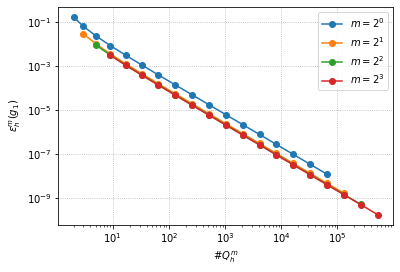
\includegraphics[width=65mm]{Aufgabe_2/latex_code/images/konvergenz_plot_5_1.png}
}
\subfloat[$a = 1$, $b = 2$]{
  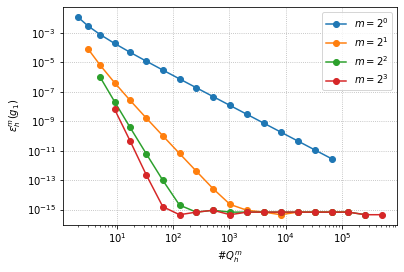
\includegraphics[width=65mm]{Aufgabe_2/latex_code/images/konvergenz_plot_5_2.png}
}
\caption{$\epsilon_\cdot^{(m)}(g_1)$, $g_1: [a, b] \to \K$, vs. $\# Q_\cdot^{(m)}$, $m = 2^r$, $r = 0, \ldots, 3$}
\label{fig:konvergenz_plot_5}
\end{figure}

Man erkennt, dass ein stumpfes Erhöhen der Anzahl der Quadraturknoten $n+1$, aufgrund der damit steigenden Anzahl der Funktionsauswertungen $\# Q_h^{(m)} = nm +1$, nicht immer sinnvoll ist. \\

Um eine bessere Approximation von $Q(f)$ zu erhalten, kann, für eine hinreichend glatte Funktionen $f$, eine höhere Quadraturformel bzw. ein höherer Extrapolationsgrad $r$, die billigere Wahl sein. Das wird durch Abbildung \ref{fig:konvergenz_plot_5} und der Potenz in \eqref{extrapolationsfehler} bestätigt. \\

Sonderfälle, wie $g_1: [0, 1] \to \K$, sind aber nicht auszuschließen. Dass sich dabei, in Abbildung \ref{fig:konvergenz_plot_5}, die Graphen verschieben, ist, aufgrund der Konstruktion der Romberg-Folge $(h_k)_{k \in \N_0}$ und dem Verhalten von $\# Q_h^{(m)}$, unmittelbar klar. Schließlich steigen beide, in $k$ bzw. $r$, exponentiell, zur Basis $2$. \\

Zuletzt wurden noch beide Extrapolationsmethoden, teuer und billig, implementiert und anhand des nicht trivialen Beispiels $\frac{\sqrt{\pi}}{2} \erf{1} = \int_0^1 \exp(-x^2) dx$ getestet. Die jeweiligen Approximationen $v_i$, und Rechenzeiten $t_i$ (in Sekunden), einer Extrapolation des Grades $r$, sind, für beide Implementierungen $i = 1, 2$, der Tabelle \ref{tab:time_table} zu entnehmen.

\begin{table}[H]
\centering
\begin{tabular}{l|l|l|l|l}
    $r$ & $v_1$ & $t_1$ & $v_2$ & $t_2$ \\
    \hline
    0  & 0.68393972058572 &  0.00011710000035 & 0.68393972058572 & 0.00004950000039 \\
    1  & 0.74718042890951 &  0.00010560000010 & 0.74718042890951 & 0.00009030000001 \\
    2  & 0.74683370984975 &  0.00045020000107 & 0.74683370984975 & 0.00019090000023 \\
    3  & 0.74682401848228 &  0.00045250000039 & 0.74682401848228 & 0.00023819999842 \\
    4  & 0.74682413309509 &  0.00107159999970 & 0.74682413309509 & 0.00022480000007 \\
    5  & 0.74682413281224 &  0.00287879999996 & 0.74682413281224 & 0.00038150000000 \\
    6  & 0.74682413281243 &  0.00366840000061 & 0.74682413281243 & 0.00047970000014 \\
    7  & 0.74682413281243 &  0.00556239999969 & 0.74682413281243 & 0.00037729999895 \\
    8  & 0.74682413281243 &  0.01505440000074 & 0.74682413281243 & 0.00065469999936 \\
    9  & 0.74682413281243 &  0.03084239999953 & 0.74682413281243 & 0.00042319999920 \\
    10 & 0.74682413281243 &  0.03871509999954 & 0.74682413281243 & 0.00046709999879 \\
    11 & 0.74682413281243 &  0.09163629999966 & 0.74682413281243 & 0.00052610000057 \\
    12 & 0.74682413281243 &  0.16136100000040 & 0.74682413281243 & 0.00059430000147 \\
    13 & 0.74682413281243 &  0.32625279999957 & 0.74682413281243 & 0.00069510000139 \\
    14 & 0.74682413281243 &  0.64237740000135 & 0.74682413281243 & 0.00083020000056 \\
    15 & 0.74682413281243 &  1.38510730000053 & 0.74682413281243 & 0.00098760000037 \\
    16 & 0.74682413281243 &  2.70271429999957 & 0.74682413281243 & 0.00156319999951 \\
    17 & 0.74682413281243 &  6.02343980000114 & 0.74682413281243 & 0.00252279999950 \\
    18 & 0.74682413281243 & 13.81374770000002 & 0.74682413281243 & 0.00591520000125 \\
    19 & 0.74682413281243 & 32.06360120000136 & 0.74682413281243 & 0.01299840000138 \\
    20 & 0.74682413281243 & 75.79247419999956 & 0.74682413281243 & 0.02835090000008
\end{tabular}
\caption{Ergebnisse $v_i$ und Rechenzeiten $t_i$ der Extrapolationsimplementierungen $i = 1, 2$}
\label{tab:time_table}
\end{table}

Tabelle \ref{tab:time_table} soll veranschaulichen, wie viel Sinn es machen kann, Funktionsauswertungen zu sparen, um ein möglichst genaues Ergebnis $v$ zu erhalten, wenn die Rechenzeit $t$ kurz sein soll.

\subsection{Nochmals die summierte Simpson- und Mile-Regel}

Der Vollständigkeit halber, berechnen wir noch die vorher benutzte summierte Simpson-Regel $Q_\cdot^{(2)}$ und summierte Mile-Regel $Q_\cdot^{(4)}$.

\begin{align*}
    Q_h^{(2)}(f)
    & = \sum_{i=1}^n Q^{(2)}(f|_{[x_{i-1}, x_i]}) \\
    & = \sum_{i=1}^n
        \frac{x_i - x_{i-1}}{6}
        \pbraces
        {
            f(x_{i-1}) +
            4 f \pbraces{\frac{x_i + x_{i-1}}{2}} +
            f(x_i)
        } \\
    & = \frac{h}{6}
        \pbraces
        {
            \sum_{i=1}^n f(x_{i-1}) +
            \sum_{i=1}^n 4 f \pbraces{\frac{x_i + x_{i-1}}{2}} +
            \sum_{i=1}^n f(x_i)
        } \\
    & = \frac{1}{3}
        \pbraces
        {
            \frac{h}{2}
            \pbraces
            {
                \sum_{i=1}^n f(x_{i-1}) +
                \sum_{i=1}^n f(x_i)
            } +
            2h \sum_{i=1}^n f \pbraces{\frac{x_{i-1} + x_i}{2}}
        } \\
    & = \frac{1}{3}
        \pbraces
        {
            Q_h^{(1)}(f) +
            2h \sum_{i=1}^n f \pbraces{\frac{x_{i-1} + x_i}{2}}
        }
\end{align*}

\begin{align*}
    Q_h^{(2)}(f)
    & = \frac{1}{3}
        \pbraces
        {
            \frac{h}{2}
            \pbraces
            {
                f(a) +
                2 \sum_{i=1}^{n-1} f(x_i) +
                f(b)
            } +
            2h \sum_{i=1}^n f \pbraces{\frac{x_{i-1} + x_i}{2}}
        } \\
    & = \frac{h}{6}
        \pbraces
        {
            f(a) +
            4 \sum_{i=1}^n f \pbraces{\frac{x_{i-1} + x_i}{2}} +
            2 \sum_{i=1}^{n-1} f(x_i) +
            f(b)
        }
\end{align*}
\begin{align*}
    & Q_h^{(4)}(f) \\
    & = \sum_{i=1}^n Q^{(4)}(f|_{[x_{i-1}, x_i]}) \\
    & = \sum_{i=1}^n
        \frac{x_i - x_{i-1}}{90}
        \pbraces
        {
            7  f(x_{i-1}) + 
            32 f \pbraces{\frac{3 x_{i-1} + x_i}{4}} +
            12 f \pbraces{\frac{x_{i-1} + x_i}{2}} +
            32 f \pbraces{\frac{x_{i-1} + 3 x_i}{4}} +
            7  f(x_i)
        } \\
    & = \frac{h}{90}
        \pbraces
        {
            7  \sum_{i=1}^n f(x_{i-1}) + 
            32 \sum_{i=1}^n f \pbraces{\frac{3 x_{i-1} + x_i}{4}} +
            12 \sum_{i=1}^n f \pbraces{\frac{x_{i-1} + x_i}{2}} +
            32 \sum_{i=1}^n f \pbraces{\frac{x_{i-1} + 3 x_i}{4}} +
            7  \sum_{i=1}^n f(x_i)
        } \\
    & = \frac{1}{15}
        \Bigg (
            \frac{7h}{6}
            \pbraces
            {
                  \sum_{i=1}^n f(x_{i-1}) +
                4 \sum_{i=1}^n f \pbraces{\frac{x_{i-1} + x_i}{2}} +
                  \sum_{i=1}^n f(x_i)
            } \\
    & +
            \frac{h}{6}
            \pbraces
            {
                32 \sum_{i=1}^n f \pbraces{\frac{3 x_{i-1} + x_i}{4}} -
                16 \sum_{i=1}^n f \pbraces{\frac{x_{i-1} + x_i}{2}} +
                32 \sum_{i=1}^n f \pbraces{\frac{x_{i-1} + 3 x_i}{4}}
            }
        \Bigg ) \\
    & = \frac{1}{15}
        \Bigg (
            7 Q_h^{(2)}(f) \\
    & +
            \frac{h}{6}
            \pbraces
            {
                32 \sum_{i=1}^n f \pbraces{\frac{3 x_{i-1} + x_i}{4}} -
                16 \sum_{i=1}^n f \pbraces{\frac{x_{i-1} + x_i}{2}} +
                32 \sum_{i=1}^n f \pbraces{\frac{x_{i-1} + 3 x_i}{4}}
            }
        \Bigg )
\end{align*}

\begin{align*}
    & Q_h^{(4)}(f) \\
    & = \frac{1}{15}
        \Bigg (
            \frac{h}{6}
            \pbraces
            {
                f(a) +
                4 \sum_{i=1}^n f \pbraces{\frac{x_{i-1} + x_i}{2}} +
                2 \sum_{i=1}^{n-1} f(x_i) +
                f(b)
            } \\
    & +
            \frac{h}{6}
            \pbraces
            {
                32 \sum_{i=1}^n f \pbraces{\frac{3 x_{i-1} + x_i}{4}} -
                16 \sum_{i=1}^n f \pbraces{\frac{x_{i-1} + x_i}{2}} +
                32 \sum_{i=1}^n f \pbraces{\frac{x_{i-1} + 3 x_i}{4}}
            }
        \Bigg ) \\
    & = \frac{h}{90}
        \pbraces
        {
            7 f(a) +
            32 \sum_{i=1}^n f \pbraces{\frac{3 x_{i-1} + x_i}{4}} +
            12 \sum_{i=1}^n f \pbraces{\frac{x_{i-1} + x_i}{2}} +
            14 \sum_{i=1}^{n-1} f(x_i) +
            32 \sum_{i=1}^n f \pbraces{\frac{x_{i-1} + 3 x_i}{4}} +
            7 f(b)
        }
\end{align*}

Die Zwischenergebnisse reflektieren das, was beim Neville-Aitken Schema \eqref{neville_aitken} passiert, wenn man die Diagonale herunterrutscht.
